% ------------------------------------------------------------------------
% file `main-bookexercise-4-solution-body.tex'
%
%     solution of type `bookexercise' with id `4'
%
% generated by the `exerciseanswer' environment of the
%   `xsim' package v0.21 (2022/02/12)
% from source `main' on 2026/10/13 on line 1519
% ------------------------------------------------------------------------
    1. 答：能确定度为0的节点有8个。哈夫曼树一定是二叉树，因此根据$n_0=n_2+1$，度为0的节点有 7 + 1 = 8个。\\

    2. 答：能确定哈夫曼树共有15个节点。由前面的讨论（参见哈夫曼树的性质，第\pageref{minisec:哈夫曼树的性质}页）可知，哈夫曼树中不存在度为1的节点，因此总节点数
    $n = n_0 + n_1 + n_2 = n_0 + n_2 = 7 + 8 = 15$。\\

    3. 略。\\

    4. 最小堆有：E、F、G；最大堆有：A、C、F。\\

    5. 选B。节点B的带权路径长度为3*1 = 3，A正确；树的带权路径长度是所有叶节点的带权路径长度之和：3*(3+1) + 2*(5+3+4) = 12 + 24 = 36，B错误；C、D显然正确。\\

    6. 显然，本题我们只要关注堆顶元素（即最小的那一个）是什么即可：
    \begin{enumerate}[label=\arabic*）]
        \item min\_heap.push(5);  // 堆中元素：5；堆顶为5
        \item min\_heap.top();    // 获取到的为5
        \item min\_heap.push(3);  // 堆中元素：5、3；堆顶为3
        \item min\_heap.push(4);  // 堆中元素：5、3、4，堆顶为3
        \item min\_heap.top();    // 获取到的为3
        \item min\_heap.pop();    // 删除堆顶元素3，4成为新的堆顶
        \item min\_heap.top();    // 获取到的为4
    \end{enumerate}

    \vspace{\baselineskip}

    7. 每次在堆中选出两个最小的来合并，计算相应体力消耗，并将合并后的新柴薪加入堆中。做n-1次即可。
    \begin{cppcode}
        int MinCost(int w[], int n) {
            priority_queue<int, vector<int>, greater<int>> min_heap;
            // 在下方完成你的代码
            int total_cost = 0;

            for(int i=0; i<n; i++) {
                min_heap.push(w[i]);
            }
            // 做n-1次
            for(int i=1; i<=n-1; i++) {
                // 取出两个重量最小的：w1和w2
                int w1 = min_heap.top();
                min_heap.pop();
                int w2 = min_heap.top();
                min_heap.pop();

                // 体力消耗为w1+w2
                int union_cost = w1 + w2;
                total_cost += union_cost;

                // 合成一堆后放回堆中
                min_heap.push(union_cost);
            }
            return total_cost;
        }
    \end{cppcode}

    \vspace{\baselineskip}

    8. 选C。哈夫曼编码，被编码的符号一定都是叶节点，又：哈夫曼树中没有只有叶节点和度为2的节点，因此有: $n_0+n_2=n_2+1+n_2=115$，得$n_2=57, n_0=58$。

    另外一种理解，生成哈夫曼树，需要合并n-1次，因此生成的度为2的节点为n-1个，代入计算也可。\\

    9. 选B。可以构造如下图所示的哈夫曼树。求出带权路径长度WPL=3*(10+12) + 2*(30+16+12) = 200。
    \begin{center}
        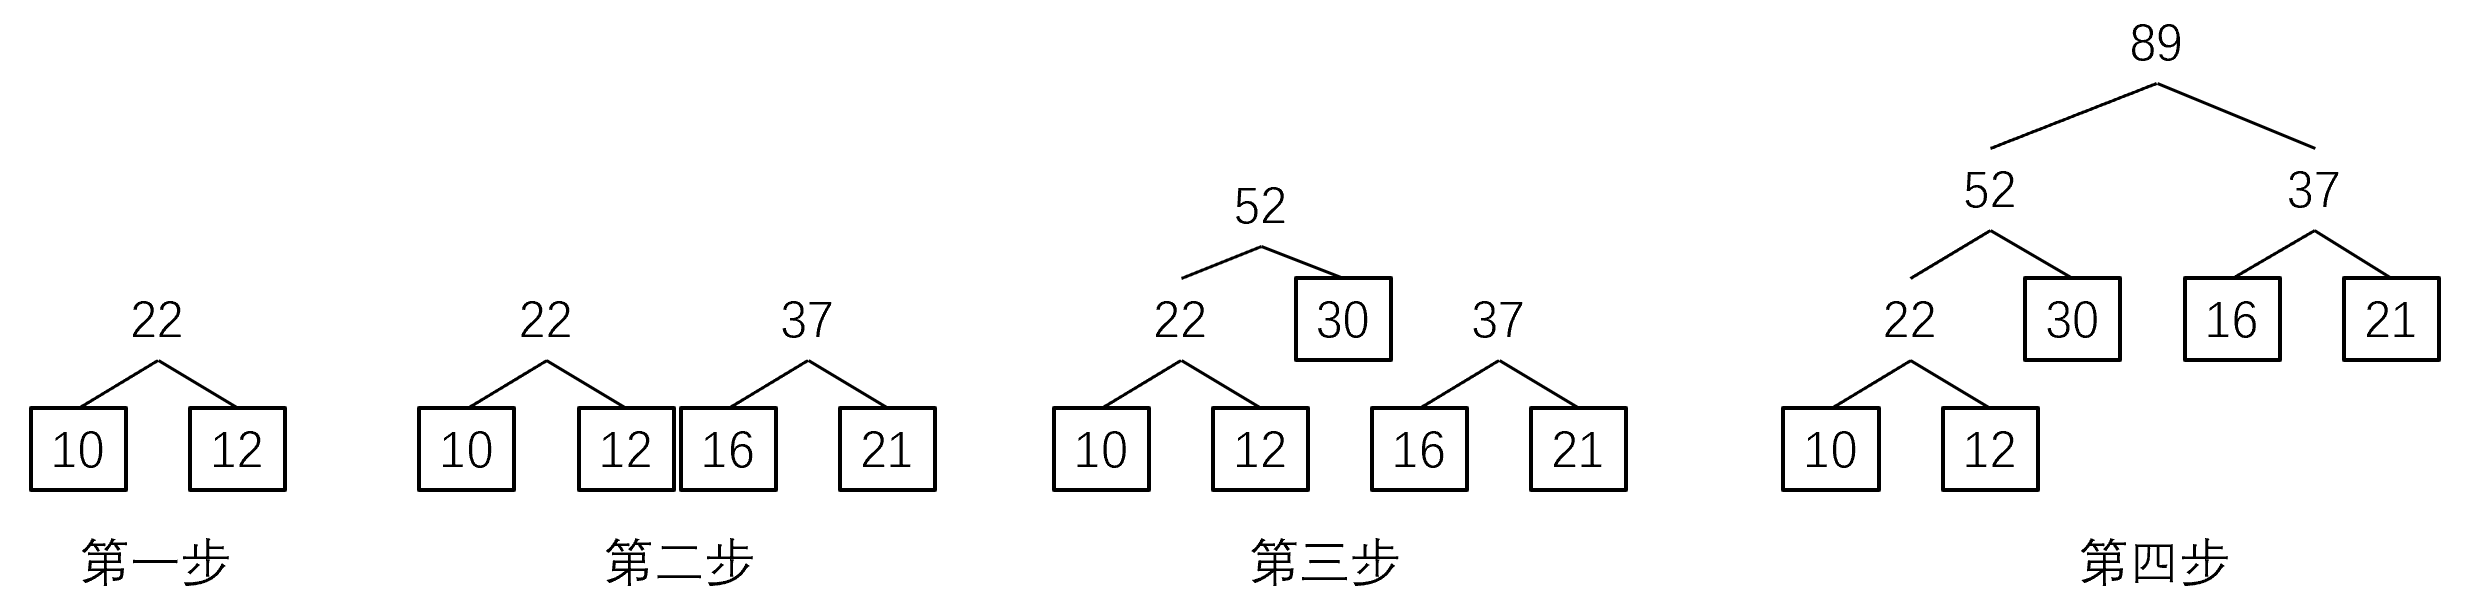
\includegraphics[width=0.89\textwidth]{assets/pics_and_ppts/ch4/21408_哈夫曼树构造过程.png}
    \end{center}

